\chapter{Javascript jako jazyk pro vývoj webových aplikací}
Javascript je skriptovací interpretovaný jazyk, jehož typickým interpretem je webový prohlížeč. Jedná se o jazyk dynamický a netypový. Umožňuje programování ve více programovacích paradigmatech například objektové, funkcionální nebo procedurální programování. Typickou vlastností javascriptového kódu je jeho asynchronní zpracování a mohutné používání událostí. Neblokující kód a událostně-orientované rozhraní je důležité při práci s uživatelskými rozhraními. Dynamičnost celého jazyka se také projevuje v možnosti přidávat, odstraňovat nebo měnit objekty za běhu programu. Ve srovnání s jinými jazyky se Javascript liší v roztříštěnosti implementací,. Existuje několik různých interpretů Javascriptu zastoupených v javascriptových jádrech jednotlivých webových prohlížečů. Nejrozšířenější implementace jsou V8 (Google Chrome), SpiderMonkey (Mozilla Firefox) nebo JScript (Internet Explorer). Společnost Microsoft nedávno uvedla novou verzi svého webového prohlížeče s požadových číslem 10, která přináší nové javascriptové jádro Chakra. Internet Explorer ale v otázce výkonu a výpočetní náročnosti stále dohání konkurenční prohlížeče \cite{zakas_js} \cite{flanagan_javascript}.
\begin{figure}[h]
\begin{centering}
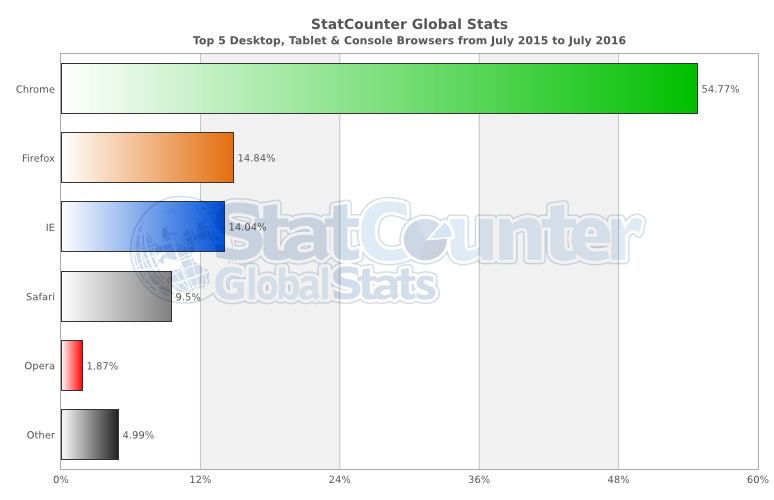
\includegraphics[scale=0.5]{obrazky/browsers}
\par\end{centering}
\caption{Zastoupení jednotlivých webových prohlížečů – červen 2016 \cite{statcounter} \label{fig:browsers}}
\end{figure}
\FloatBarrier
Syntaxe jazyka Javascript, pocházející z rodiny jazyků C++ a Java, je velkou výhodou pro vývojáře, kteří s ním začínají. Základním konstruktem Javascriptu je objekt, který reprezentuje všechny neprimitivní typy. Nezbytnou součástí jazyka je \textit{funkce}. Funkce je také instance typu Object a je možné s ní manipulovat jako s jakýmkoliv jiným objektem. Javascript implementuje takzvané \uv{first-class citizen funkce (prvotřídní funkce)}. To znamená že funkci lze uložit do proměnné a pracovat s ní jako s jakýmikoliv jinými daty \cite{flanagan_javascript}. Prvotřídní funkce je základním předpokladem pro funkcionální programování, které je pro javascript typické. Jeho funkcionální podstata dovoluje velice snadno vytvářet asynchronní anonymní funkce, které jsou pak registrovány jako obslužné funkce pro události. Událostí může být kliknutí uživatele na tlačítko, změna obsahu formulářového prvku, nebo načtení nové stránky. Pomocí protypové dědičnosti a takzvaných konstrukčních funkcí je také možné programovat do značné míry objektově. Javascript je implementovaný ve všech hlavních desktopových i mobilních webových prohlížečích a pomocí node.js jej lze provozovat i na serveru \cite{flanagan_javascript} \cite{hronek_javascript}. Jak lze vidět na následujícím grafu, Javascript je v současné době čtvrtým nejpoužívanejším jazykem \cite{skriptovaci_jazyky}. Také na serveru Github, který sdružuje git repozitáře zdrojového kódu má aktuálně (2016) Javascript nejvíce aktivních repozitářů, což vedle oblíbenosti tohoto jazyka, značí také ochotu javascriptových vývojářů uvolnit svůj kód jako open source \cite{githut}.
\vspace{0,3cm}
\begin{figure}[h]
\begin{centering}
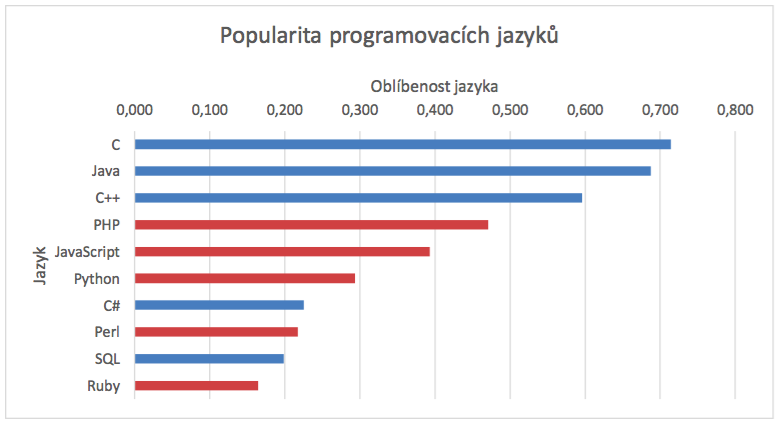
\includegraphics[scale=0.5]{obrazky/popularita_jazyku}
\par\end{centering}
\caption{Grap popularity programovacích jazyků, červeně označené skriptovací jazyky \cite{skriptovaci_jazyky} \label{fig:language-preferences}}
\end{figure}

\section{Historický vývoj}
Původní koncepce webových stránek nepočítala s použitím žádného programovacího jazyka, znala pouze HTML jako značkovací a CSS jako stylovací jazyk. Až v roce 1995 Brendan Eich představuje jazyk LiveScript, když pro společnost Netscape vymýšlí skriptovací jazyk, který chce firma využívat ve svém webovém prohlížeči. Firma krátce před jeho vydáním rozhodně o změně názvu na JavaScript\footnote{Dnes je rozšířenější označení Javascript, s malým \uv{s}, které budu používat i v této práci.}, kvůli tehdejší popularitě jazyka Java. Brzy po vydání první verze prohlížeče Netscape Navigator, přichází také společnost Microsoft se svým prohlížečem Internet Explorer. Ten také ve své verzi 3, vydané v roce 1996, podporoval Javascript, ačkoli byl jeho interpret kvůli obavám z licenčních sporů pojmenován jako JScript. Objevily se také některé další prohlížeče, které také dokázaly zpracovávat Javascript. V jednom okamžiku tedy existovalo několik rozdílných intepretů Javascriptu, což vynutilo potřebu standardizace tohoto jazyka. Byla založena organizace ECMA a vydán nový standard ECMA–262, který definoval skriptovací jazyk ECMAScript. Ten se stal základem pro různé implementace Javascriptu používané v různých webových prohlížečích. Javascript, který známe dnes, je také pouze jednou z implementací standardu ECMAScript. Díky jeho obrovské popularitě se ovšem tyto dva termíny často libovolně zaměňují. Existují však ještě další implementace jako JScript či ActionScript \cite{zakas_js} \cite{flanagan_javascript} \cite{hronek_javascript} .

Jednotlivé verze standardu ECMA se nazývají \textit{edice}, ta stále aktuální vyšla v červnu 2001 a nese označení 5.1 (dnes často nazývána ES5), v dnešních dnech (2016) je téměř dokončen přechod na verzi ES6, vydanou v roce 2015. Také byly záhájeny práce na vývoji další verze s pořadovým číslem sedm, která je očekávána v roce 2017. Některé nové vlastnosti ES7 jsou už implementovány v posledních verzích prohlížečů Mozilla Firefox a Google Chrome. Javascript se stal použitelnějším jazykem díky vývoji výkonných javacriptových běhových prostředí zejména ze strany společností Google a Mozilla \cite{hronek_javascript} \cite{ecmascript}. 
Na obrázku níže můžeme vidět běžné typy architektur webových aplikací, spolu s jejich výhodami a nevýhodami.
\begin{figure}[h]
\begin{centering}
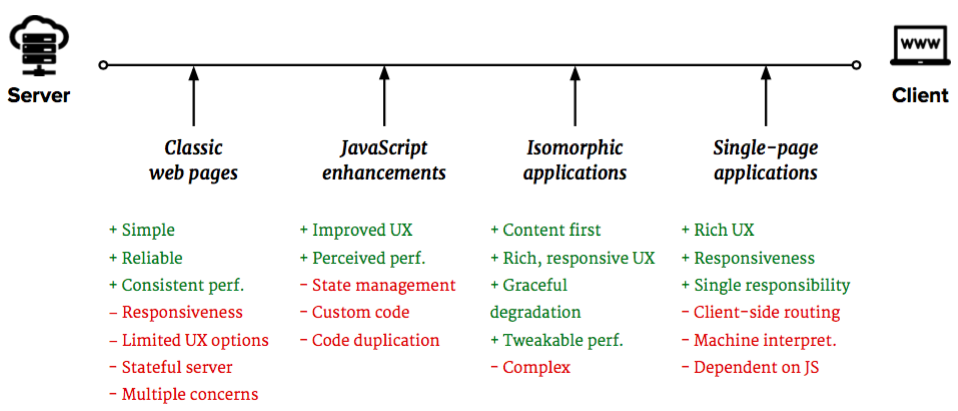
\includegraphics[scale=0.4]{obrazky/websites}
\par\end{centering}
\caption{Diagram typických architektur webových aplikací \cite{codepicnic_universaljs} \label{fig:typical-web-arch-diagram}}
\end{figure}
\FloatBarrier

\section{ES6 – Nové standardy}
Standard ES6, který definoval moderní podobu jazyka Javascript vyšel v srpnu 2015. Implementace standardů je však zdlouhavý proces, takže i když je standard ES6 téměř rok vydaný, kompletní podpora stále není implementována ve všech prohlížečích. Největší problém je tradičně u Internet Exploreru, kde i ten nejnovější jedenáctý ES6 téměř vůbec nepodporuje. V jiných prohlížečích se ES6 už těší velmi slušné podpoře. Potíž je však v tom, že ne všichni uživatelé používají poslední verze prohlížečů. V praxi je tak potřeba se ES6 zatím úplně vyhnout, nebo použít nějaký javascriptový transpiler (viz. \hyperref[sec:js_transpilers]{2.3}). Lepší situace je u node.js, kde poslední šestá verze má už 93\% podporu ES6 (viz. \hyperref[sec:node_js]{2.4}). Změnil se také proces, podle něhož se budou dostávat nové věci do prohlížečů. Vývoj standardu ES6 trval dlouhých 6 let, proto bylo nutné také navrhnout postup dalšího vývoje \cite{exploring_es6}. Nyní bude vznikat každý rok nová verze standardu ECMAScript \cite{tc39ecma}. Následuje přehled nejzajímavějších novinek nového standardu jazyka Javascript \cite{exploring_es6}.

\subsection{Třídy}
S nutností alespoň částečně používat Javascript téměř u každé webové aplikace, začalo tento jazyk používat stále více typických objektově orientovaných programátorů. Ti se snažily používat principy objektového návrhu i v Javascriptu. Základním kamenem objektového přístupu je \textit{třída}, kterou ale Javascript vůbec nezná. Také nezná klasickou dědičnost, místo toho obsahuje takzvanou protypovou dědičnost. Ta zjednoduše řečeno umožňuje definovat prototyp, ze kterého bude každý objekt daného typu vytvořen. Až standard ES6 přináší nové klíčové slovo \textit{class}, které usnadňuje objektově orientované programování v jazyce Javascript. Je již tedy možné definovat třídu, její kontruktor, provádět volání rodičovské metody nebo implementovat statické metody. Je také možné dědit jinou třídu pomocí klíčového slova \textit{extends}, které realizuje již zmíňenou prototypovou dědičnost na pozadí. Mnoho zkušenejších javascriptových vývojářů ale zastává názor, že přidání této syntaxe je velká chyba. Bude totiž svádět vývojáře ke klasickému OOP, což je v Javascriptu z mnoha důvodů považováno za špatné \cite{exploring_es6} \cite{es6} \cite{es6_book}.
\begin{lstlisting}[language=Javascript,caption={Ukázka ES6 syntaxe pro třídy v Javascriptu \cite{es6}}]
class SkinnedMesh extends THREE.Mesh { // definice třídy
  constructor(geometry, materials) { // konstruktor
    super(geometry, materials);

    this.idMatrix = SkinnedMesh.defaultMatrix();
    this.bones = [];
    this.boneMatrices = [];
    //...
  }
  update(camera) { // třídní metoda
    //...
    super.update();
  }
  static defaultMatrix() { // statická metoda
    return new THREE.Matrix4();
  }
}
\end{lstlisting}

\subsection{Let a const}
\label{sec:variable_scope}
Jednou z nejkritizovanějších vlastností jazyka Javascript je globální kontext všech funkcí a proměnných. Definování proměnné na jakémkoliv místě znamená její uložení do globálního kontextu aplikace. Opětovné definování proměnné pod stejným názvem neskončí chybou, ale přepsáním původní hodnoty. To může přinášet nečekané problémy například nováčkům. Ovšem jako u každé nevýhody Javascriptu, našla komunita několik běžně používaných řešení. Nejčastěji se jedná o obalení kódu javascriptovou anonymní funkcí, které je vykonána ihned po deklaraci. Jedná se o takzvanou IIFE (Immediately-Invoked Function Expression) \cite{exploring_es6} \cite{es6} \cite{es6_book}.

\begin{lstlisting}[language=Javascript,caption={IIFE – řešení lokálního kontextu v ES5 Javascriptu. \cite{exploring_es6}}]
(function () {  // začátek IIFE
    var tmp = "something";
}());  // ukončení a zavolání IIFE

console.log(tmp); // ReferenceError, tmp není na globálním kontextu definováno
\end{lstlisting}

ES6 ovšem problém globálního kontextu řeší zavedením nových klíčových slov \textit{let} a \textit{const}. Příkaz let oproti běžnému var omezuje kontext proměnné na nejbližší blok. Const definuje neměnitelnou konstantu \cite{exploring_es6} \cite{es6} \cite{es6_book}.
\begin{lstlisting}[language=Javascript,caption={Ukázka nových klíčových slov pro proměnné v ES6 Javascriptu \cite{exploring_es6}.}]
function fn() {
  {
    let x;
    {
      // platnost pouze v tomto bloku
      const x = "sneaky";
      // chyba, nemůžeme měnit konstantu
      x = "foo";
    }
    // chyba, nemůžeme opět deklarovat x ve stejném bloku
    let x = "inner";
  }
  console.log(x); //ReferenceError není definováno na tomto bloku
}
\end{lstlisting}
\subsection{Moduly}
Nezbytnou vlastností každého moderního programovacího jazyka je podpora modularizace, původní Javascript podle očekávání žádnou vestavěnou podporu nemá. Nezná ani klíčové slovo \textit{include}. Bylo tedy nutné přinést nějaké řešení, dnes existuje několik konvencí pro javascriptové moduly jako Common.js, AMD nebo UMD. Ty popisují API, která zaručují správnost jeho načtení a následné komunikace. Samotná modularizace je také často v Javascriptu realizována pomocí vlastních kličových slov (například \textit{require()}), postprocesor potom spojí jednotlivé moduly v jeden velký javascriptový soubor, ze kterého je potom celá aplikace spuštěna. Nejznámější z nich je \textit{browserify} nebo také čím dál oblíbenejší \textit{webpack}. Postprocessor prochází soubory webové aplikace počínaje výchozím bodem (entrypointem) aplikace a hledá v nich deklarace závislostí na dalších souborech. Tento přístup zajišťuje použití jen skutečně využívaného kódu. V dřívejších dobách obsahoval každý postprocesor pro definici zdrojů vlastní syntaxi, dnes se téměř výhradně používá syntaxe dle ES6. Standard ES6 totiž přináší nové klíčové spolo \textit{import}, které dodává do Javascriptu tolik postrádanou možnost načítání externích zdrojů. Načítání může být konečně řešeno na straně jazyka a není nutné ho realizovat pomocí specializovaných nástrojů. Mechanismus sestavení jednoho výstupního souboru obsahujícího celou aplikaci však zůstal zachován, je nutný pro zmenšení datové náročnosti a počtu dotazů výsledné webové aplikace \cite{exploring_es6} \cite{es6} \cite{es6_book}. Následuje popis nových klíčových slov jazyka Javascript usnadňujících práci s moduly.

\vspace{3mm}
Ze souboru můžeme exportovat funkce, objekty i proměnné pomocí klíčového slova \textit{export} \cite{es6}.
\begin{lstlisting}[language=Javascript,caption={Deklarace modulu v ES6 Javascriptu \cite{es6}}]
// lib/math.js
export function sum(x, y) {
  return x + y;
}
export var pi = 3.141593;
\end{lstlisting}

V jiném souboru si je pak můžeme importovat pomocí klíčových slov \textit{import} a \textit{from}. Použijeme-li znak hvězdičky (*) naimportujeme z externího souboru vše. Můžeme si ale i vybrat, které části modulu potřebujeme pomocí \textit{destructuringu} (viz níže) \cite{exploring_es6} \cite{es6} \cite{es6_book}.
\begin{lstlisting}[language=Javascript,caption={Použití modulu v ES6 Javascriptu \cite{es6}}]
// app.js
import * as math from "lib/math"; //import všeho z lib/math.js
alert("2pi = " + math.sum(math.pi, math.pi)); // přibyl nový objekt math

import {sum, pi} from "lib/math"; //import jen některých částí z lib/math.js
alert("2pi = " + sum(pi, pi)); // na lokálním kontextu přibyly nové objekty sum a pi
\end{lstlisting}
Specialitou je nové klíčové slovo \textit{default}. To definuje, která část souboru se importuje, není li explicitně řečeno která část se má použít. V cílovém souboru si můžeme default import pojmenovat zcela dle své vůle (zde exp). Současně můžeme i nadále importovat ostatní funkce, objekty a proměnné \cite{exploring_es6} \cite{es6} \cite{es6_book}.
\begin{lstlisting}[language=Javascript,caption={Použití modulu s klíčovým slovem default v ES6 Javascriptu \cite{es6}}]
// lib/mathplusplus.js
export * from "lib/math";
export var e = 2.71828182846;
export default function(x) {
    return Math.exp(x);
}

// použití
// app.js
import exp, {pi, e} from "lib/mathplusplus";
alert("2pi = " + exp(pi, e));
\end{lstlisting}

\subsection{Další novinky}
Standard ES6 přinesl také mnoho dalších novinek, velmi užitečné jsou výchozí hodnoty argumentů funkcí, šablony pro řetězce nebo destructuring. Dále naleznete ukázky použití posledních dvou zmíněných novinek: šablon pro řetězce, které se uvozují takzvaným \textit{backtick operátorem} ( {\large \textbf{`}} ) a \textit{destructuringu}. Ten umožňuje využít jen některé exportované části importovaného modulu. Často se používá pro získání jen některých funkcí nějaké externí knihovny, například hypotetický zápis \textit{const \{ajax,cookies\} = angular} by získal z frameworku AngularJS jenom moduly zodpovědné za podporu AJAX operací a správu cookies \cite{exploring_es6} \cite{es6} \cite{es6_book}.

\begin{lstlisting}[language=Javascript,caption={Ukázka použití šablon pro řetězce v ES6 \cite{exploring_es6}. }]
//ES5 syntaxe
function printCoord(x, y) {
    console.log('(X='+x+',Y= '+y+')');
}
//ES6 syntaxe
function printCoord(x, y) {
    console.log(`(X=${x}, Y=${y})`);
}

\end{lstlisting}

\begin{lstlisting}[language=Javascript, caption={Ukázka použítí destructuringu v ES6 \cite{exploring_es6}}]
const obj = { first: 'Jane', last: 'Doe' };
const {first, last} = obj;
    // first = 'Jane'; last = 'Doe'
\end{lstlisting}

\section{Javascriptové transpilery}
\label{sec:js_transpilers}
Standard ES6 přináší dva základní typy novinek.  První jsou nová rozhraní nebo rozšíření těch existujících, tyto změny můžeme ve starším Javascriptu simulovat pomocí mnoha knihoven, které se nazývají shimy nebo polyfilly. Ty dokážou detekovat podporu moderního Javascriptu a případné chybějící funkce doplnit. V budoucnu, až bude většina používaných webových prohlížečů plně podporovat ES6, mohou být tyto knihovny odstraněny. Druhou novinkou je nová syntaxe, například nová klíčová slova \textit{class}, \textit{extends}, \textit{let} či \textit{import}. Změny v samotné syntaxi Javascriptu již nejde simulovat nějakou knihovnou, je nutné používat program – kompilátor, který náš kód přeloží do aktuálně plně podporované verze Javascriptu, tedy do ES5. Protože se jedná o převod mezi programovacími jazyky stejné úrovně, používá se označení \textit{transpiler} nebo \textit{source-to-source kompilátor}. Zpětný překlad není většinou možný. Javascriptový transpiler, mimo převodu kódu na starší verzi, provede také doplnění všech nutných polyfillů, aby byla zajištěna funkčnost na většině současných prohlížečů \cite{learning_es6} \cite{transpilers}.

Jedná se o stejný přístup jako u kompilátorů skriptovacích jazyků, které jsou do Javascriptu překládány. Z nejznámějších lze zmínit CoffeeScript nebo Purescript. Tyto jazyky vznikly před příchodem ES6, aby syntakticky zjednodušily vývoj v Javascriptu. Dnes je doporučované používat ES6 a oblíbenost těchto jazyků začíná klesat. Javascriptové transpilery lze tedy rozdělit do dvou základních kategorií. První jsou zcela nové jazyky, které mají úplně odlišnou syntaxi a nemůžeme je tedy použít na vylepšení již hotových projektů. Druhou představují jazyky, které Javascript jen rozšiřují a snaží se zachovat maximální dopřednou kompatibilitu. Mezi takové řadíme i BabelJS \cite{babel}, který je popsán níže \cite{learning_es6} \cite{transpilers}.

\begin{enumerate}
\item \textbf{používající vlastní vstupní jazyk} – CoffeeScript, PureScript, Script\#, Haxe
\item \textbf{kompilující moderní Javascript do současného} – Babel, TypeScript, Traceur 
\end{enumerate}

\subsection{CoffeeScript}
CoffeeScript je nový programovací jazyk, který se kompiluje do Javascriptu. Byl vytvořen pro zjednodušení syntaxe původního Javascriptu, odstraňuje z něj středníky, závorky a také zavádí definici tříd typickou pro objektově orientované jazyky. Při svém vývoji byl inspirován syntaxí jazyka Ruby, ve kterém byl napsán i první překladač, současné verze překladače je již napsána v Javascriptu, respektive samotném CoffeeScriptu. První verze byla vydána v roce 2009 a jeho autor Jeremy Ashkenas do první commit message napsal: \uv{initial commit of the mystery language}, což lze přeložit jako první commit záhadného jazyka \cite{coffeescript_founder}. První stabilní verze vyšla na Vánoce roku 2010. CoffeeScript se běhěm několika let stal velmi populárním. Někteří vývojáři však zastávají názor, že zjednodušení syntaxe naopak zhoršilo čitelnost výsledného kódu. Velkou nevýhodou je špatné odhalování programátorských chyb, protože chyba se zobrazí ve vygenerováném javascriptovém kódu. Až po jejím pochopení je možné ji dekódovat na úrovni CoffeeScriptu. Na druhou stranu ke každému kódu v CoffeeScriptu existuje ekvivaletní kód v Javascriptu, a proto lze při vývoji používat jakékoliv javascriptové knihovny \cite{coffeescript}.

\begin{table}[h]
\centering
	\caption{Ukázka syntaxe CoffeeScriptu spolu s překladem do Javascriptu \cite{coffeescript} \label{fig:js_vs_coffee}}
	\begin{tabular}{ |p{5cm}|p{5cm}| }
	\hline
	CoffeeScript & Javascript \\ \hline
	number = -42 if opposite & 
	\begin{minipage}[t]{0.2\columnwidth}%
       if(opposite)\{
          \newline
          number = -42;
          \newline
          \}
    \end{minipage}	
	\\ \hline
	squere = (x) -> x * x &	
	\begin{minipage}[t]{0.2\columnwidth}%
       var square = function(x) \{
          \newline
          return x * x;
          \newline
          \};
    \end{minipage}
    \\ \hline
    alert "I knew it!" if elvis? &
    \begin{minipage}[t]{0.4\columnwidth}%
       if(typeof elvis !=="undefined" 
          \newline
          \&\& elvis !==null)\{
          \newline
          alert("I knew it!");
          \newline
          \}
    \end{minipage}
    \\ \hline
	\end{tabular}
	\label{tab:coffeescript}
\end{table}

\subsection{Babel}
\label{sec:babel}
Aby bylo možné používat Javascript ES6 už dnes a nečekat několik let než se dostane alespoň do posledních verzí prohlížečů, vznikl projekt Babel. Ten představuje transpiler ES6 kódu do verze ES5, kterou umí většina současných prohlížečů. Babel vznikl v roce 2015 jako projekt 6to5 a rychle si získal velkou oblíbenost mezi javascriptovými vývojáři a jeho využití stále stoupá. Hlavním důvodem je nejširší podpora standardu ES6 včetně některých nových vlastností ES7. Babel také plně integruje JSX a je tedy více než vhodný pro použití s frameworkem React. Příchod Babelu bude také nejspíš znamenat snižování ochoty vývojářů používat jiné jazyky, které se kompilují do Javascriptu, protože bude jistější používat něco, co je standardizované než vlastní jazyk vymyšlený nějakou společností nebo vývojářem. Babel lze také používat v node.js, i když tempo zavádění ES6 do node.js je výrazně rychlejší než u webových prohlížečů. Kvůli různým javascriptových prostředím, kde cílový kód poběží, obsahuje Babel takzvané \uv{presety}. Pomocí nichž lze nastavit na jakou verzi Javascriptu má provést překlad kódu, které lze rozdělit na dvě základní skupiny. Prvním skupinou jsou webové prohlížeče. Zde záleží především na potřebě kompatibility aplikace s prohlížečem Internet Explorer. Druhou skupinou je node.js, kde každý preset odráží novou verzi tohoto frameworku. V budoucnu až node.js tým dokončí plnou implementaci standardu ES6, nebude využití Babelu v node.js nutné. Výběr vhodného presetu je na vývojáři, který musí zvážit jaké prohlížeče ještě chce podporovat a jaké už ne. Knihovna Babel ve výchozím stavu kompiluje Javascript kompletně do ES5, výsledek by měl být funkční ve většině současných prohlížečů počínaje Internet Explorerem 9 \cite{babel} \cite{babel_what}. Následuje ukázka konverze nového zápisu pro funkce z ES6.
\vspace{0,3cm}
\begin{figure}[h]
\begin{centering}
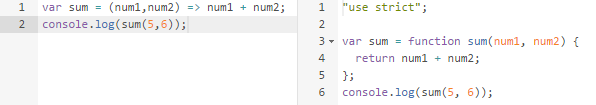
\includegraphics[scale=0.6]{obrazky/babel}
\par\end{centering}
\caption{Ukázka konverze ES6 javacriptu do ES5 pomocí transpileru Babel \cite{babel} \label{fig:babel}}
\end{figure}
\FloatBarrier

Babel dnes používají největší internové společnosti jako Facebook, Yahoo, Netflix, Mozilla nebo Evernote \cite{babel}.

\section{Node.js – Javascript na serveru}
\label{sec:node_js}
Důležitým pokrokem ve světě Javascriptu bylo představení platformy Node.js, která umožnila spouštění javascriptového kódu na serveru. S nárůstem oblíbenosti tohoto jazyka jistého člověka napadlo vzít javascriptové jádro V8 z prohlížeče Google Chrome a postavit nad ním velmi výkonnou platformu, použitelnou i mimo webový prohlížeč, zejména na serverech. Tím člověkem byl Ryan Dahl a celá platforma, která byla navržena s ohledem na dobrou škálovatelnost vycházející z principu asynchronního zpracování kódu v jednom vlákně, byla v roce 2009 uvolněna jako open source. Engine V8, napsaný v C++, kompiluje Javascriptový kód do nativního a nejen díky tomu je jedním z nejvýkonnějších javascriptových enginů. Tím pádem bylo jeho použití ideální. Jeho nápad se setkal s obrovským ohlasem a dnes node.js tvoří nepostradatelnou část javascriptového ekosystému. Node.js je zaměřené na dlouhodobě běžící serverové procesy, na rozdíl od jiných prostředí ale neumí využívat více vláken najednou (multithreading). Místo toho využívá čistě asynchronní povahu jazyka Javascript a veškeré operace provádí v jednom hlavním vlákně. Server se tedy chová jako démon\footnote{Termínem démon se v IT prostředí označuje specifický program, který svou činnost provozuje dlouhodobě a vůbec nemusí být nijak závislý na přímém kontaktu s koncovým uživatelem (jejich vzájemné interakci).} spouštějící javascriptový interpret. V poslední době se však objevují snahy vícevláknové operace do node.js doplnit \cite{nodejs} \cite{glover_nodejs} \cite{tilkov_nodejs}.

\begin{lstlisting}[language=Javascript,caption=Ukázka kompletní implementace programu Hello World v node.js]
var http = require('http');
http.createServer(function (request, response) {
    response.writeHead(200, {'Content-Type': 'text/plain'});
    response.end('Hello World\n');
}).listen(8000);

console.log('Server running at http://localhost:8000/');
\end{lstlisting}

Výše uvedený příklad kódu je kompletní implementací webového serveru, zobrazujícího text \textit{Hello World} v node.js. Na prvním řádku můžeme vidět získání závislosti na webovém serveru, pro které má node.js speciální funkci \textit{require}. Funkcionální přístup javascriptu je pro úlohy jako webové server ideální, ukázkový kód je proto velmi krátký. V lednu 2010 byl také přestaven balíčkovací systém \textit{npm}, který řeší správu, instalaci a aktualizaci javascriptových balíčků. Z počátku byl používán jen pro node.js, v současnosti již proniká i do vývoje frontendových částí aplikací, tedy do webových prohlížečů. Dnes má npm více než 250 000 stažených balíčků každý den \cite{nodejs_numbers}. Každá aplikace využívající pro zprávu závislostí npm obsahuje v hlavním adresáři soubor \textit{package.json}, který definuje celou npm aplikaci. Tento soubor obsahuje popisná data o aplikaci, závislosti na externích knihovnách včetně verzí (je možné definovat také závislosti určené jen pro vývoj), umístění repozitáře, vstupní bod aplikace nebo například typ licence. Npm je kompletně ovládáno z příkazové řádky. Pomocí příkazu \textit{npm install} dojde \uv{nainstalování}  aplikace, jsou tedy staženy a nainstalovány veškeré závislosti a aplikace připravena ke spuštění. Npm také nově umožňuje definici úkolů pro vestavěný task runner (viz \hyperref[sec:task_runner]{2.6}), kterým lze webovou aplikaci dále spravovat \cite{glover_nodejs} \cite{tilkov_nodejs} \cite{npm}.

\begin{lstlisting}[language=Javascript, caption=Soubor package.json definující závislosti pro NPM]
{
  "name": "amazing-js-app",
  "version": "0.2.0",
  "description": "A amazing js app written in Javascript",
  "main": "index.js", //vstupní bod aplikace
  "scripts": {
    "start": "node index.js" // úkoly pro task runner
  },
  "dependencies": { // zavislosti
    "express": "^4.13.3"
    ...
  },
  "devDependencies": { //zavislosti pro vývoj
    "mocha": "^4.13.3"
    ...
  },
  "repository": { //umístění repozitáře
    "type": "git",
    "url": "https://github.com/jakub.josef/amazing-js-app"
  },
  "keywords": [
    "amazing",  "js",  "app"
  ],
  "author": "Jakub Josef",
  "license": "MIT"
}
\end{lstlisting}

I když není ještě zastoupení javascriptových serverů příliš vysoké, tento trend již několik let roste. Dle Tilkov, Vinosky pro to existuje několik hlavních důvodů. Jedním z nich je nástup technlogií pod značkou HTML5, které vytlačují alternativní platformy na straně klienta, jako například Adobe Flash nebo Microsoft Silverlight, kde je nutné použít Javascript. Je pak více než vhodné použít stejný jazyk i na serveru \cite{tilkov_nodejs}.

Zajímavou knihovnou je také Electron, přes který lze psát pomocí node.js klasické desktopové aplikace a je v něm napsaný třeba textový editor Atom.io nebo klient pro komunikátor Slack \cite{elektron}. 

\section{Vývojové nástroje}
S nárůstem oblíbeností Javascriptu vzniklo obrovské množství knihoven\footnote{Občas se objevují pokusy rozlišit termíny knihovna a framework, v této práci budou používány víceméně ekvivalentně.} a nástrojů, které usnadňují proces vývoje. Typické vývojové prostředí se skládá s desítek knihoven usnadňující práci se šablonami, získávání dat nebo testování. Je tedy nutné používat nějaký skript nebo program, který bude celé vývojové prostředí řídit. Ve světě Javascriptu se příliš neuchytilo používání velkých IDE\footnote{Integrated Development Environment – kompletní vývojářské prostředí, například Eclipse, Intellij IDEA nebo Netbeans IDE}. Místo toho se využívá takzvaných \textit{task runnerů}, kteří mají definovány relevantní úkoly, například sestavit aplikaci a spustit vývojový webový server, aktivovat testy, nebo vytvořit balíček pro produkční nasazení. Task runner se zpravidla ovládá pomocí příkazové řádky. Typické vývojové prostředí je pro moderní aplikace v Javascriptu velmi komplexní a jeho prvotní konfigurace může být složitá. Je to proto, že na takové prostředí jsou dnes kladeny vysoké požadavky. Jsou to například: \cite{flanagan_javascript} \cite{task_runners} 

\vspace{0.5cm}
\begin{itemize}
\item programování v ES6 Javascriptu, možnost použití transpileru,
\item škálovatelnost výsledné aplikace,
\item maximální modularita,
\item možnost jednoduše integrovat a používat stovky tisíce balíčků z npm,
\item používat nějaký CSS preprocesor, 
\item po každé změně v kódu by měl být ihned vidět výsledek v prohlížeči (livereload),
\item vývojový a produkční mód,
\item v produkčním módu všechny potřebné JS soubory (moduly) sloučit do jednoho a minimalizovat, obdobně i pro kaskádové styly,
\item v produkčním módu ignorovat warningy a jiné debugovací výpisy,
\item kontrola (lintování) kódu,
\item spouštění testů uvnitř webového prohlížeče.
\end{itemize}

\section{Automatizace vývoje}
\label{sec:task_runner}
Jak je již zmíněno, vývojové prostředí většinou obsahuje větší množství knihoven a nástrojů, jejichž vzájemnou interakci řeší task runner. Ten umožňuje definovat úkoly (tasky), které provedou nějakou činnost. Typicky se jedná například o minifikaci JS kódu nebo obsluhu vývojového webového serveru. Tomuto přístupu se říká \textit{automatizace vývoje} a je ve světě moderního Javascriptu naprosto zásadní. Prvním populárním programem tohoto typu byl \textit{Grunt} \cite{grunt}, dnes je mezi vývojáři oblíbenější jeho přímý konkurent Gulp, který je použit i v této práci. Gulp vyniká především jednodušší konfigurací a větším výkonem \cite{gulp}. Většinu takových úkolů pro běžně používané knihovny není nutné programovat, lze je nalézt v balíčkovacím systému NPM, a to pro oba zmíněné automatizační nástroje. Úkoly je do sebe možné libovolně zanořovat a volat je v určeném pořadí.  Je také možné použít připravené vývojové prostředí, takzvaný \uv{devstack}. Ten obsahuje mnoho hotových úkolů, usnadňujících vývoj. Jejich použítí je dnes doporučované, existují desítky devstacků pro všechny nejpoužívanější javascriptové webové frameworky \cite{task_runners}. Představení několika z nich naleznete v kapitole \hyperref[sec:devstacks]{4.6}.

\vspace{3mm}
\noindent Task runner Gulp ukládá konfigurace do souboru Gulpfile.js \cite{gulp} \cite{gulp_web}. Následující ukázka kódu demonstruje jednoduchost jeho konfigurace.

\begin{lstlisting}[language=Javascript,caption={Ukázka konfigurace task runneru Gulp \cite{gulp}}]
// načtení externích knihoven
var gulp = require('gulp')
, fs = require('fs')
, coffeelint = require("gulp-coffeelint")
, coffee = require("gulp-coffee")
, uglify = require("gulp-uglify")
, concat = require("gulp-concat")
, header = require("gulp-header");
 
// definice úkolu bundle
gulp.task('bundle', function () {
    gulp.src('./coffee/*.coffee') // cesta ke zdrojovým souborům
    .pipe(coffeelint()) // lintování
    .pipe(concat('bundle.js')) // spojení souborů do jednoho s názvem bundle.js
    .pipe(coffee()) // kompilace CoffeeScriptu
    .pipe(uglify()) // minifikace zkompilovaného Javascriptu
    .pipe(gulp.dest('./dist')); // uložení do adresáře dist
});
\end{lstlisting}

Task runner Gulp je hluboce založen na takzvaných streamech (česky datových proudech), každý stream provádí vždy určitou činnost, na vstup přijímá cestu k souboru nebo jiný stream a jeho výsledky mohou být zapsány do souboru nebo předány dalšímu streamu \cite{gulp_web}. Výše uvedená konfigurace definuje úkol (task) \textit{bundle}, který provede následující v daném pořadí:
\begin{enumerate}
\item načtení CoffeeScript kódu z adresáře coffee
\item kontrola (lintování) CofeeScript kódu
\item spojení všech souborů v jeden
\item kompilace CoffeeScriptu
\item minifikace (odstranění mezer a zkrácení kódu) vygenerováno Javascriptu
\item uložení výsledku do adresáře dist
\end{enumerate}

\section{Lintování kódu}
Takzvané \uv{lintování} kódu je proces, který pomáhá sjednotit vzhled a zajistit formální správnost zdrojového kódu celé aplikace. Program, který tyto kontroly provádí se nazývá linter. Ten hlídá styl kódu, korektní používání závorek či odsazení. Pravidla, kterými se řídí jsou dány aktuálními standardy v lintovaném jazyce, ty je možné upravit, nebo si definovat vlastní. Linter také umí odhalit některé překlepy nebo nepoužívané konstrukce. Pro jazyk Javascript se dlouhou dobu používal nástroj JSHint, který dnes nahrazuje ESLint, který přináší především podporu modularity. Je tedy možné jej rozšířit o validování Babel syntaxe nebo JSX komponent z frameworku React. Lintování kódu bývá zpravidla součástí build procesu, aby se odhalily nedostatky před vytvořením nové verze aplikace \cite{flanagan_javascript} \cite{linter}.

\begin{figure}[h]
\begin{centering}
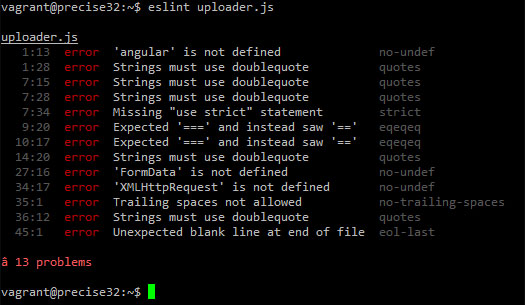
\includegraphics[scale=0.6]{obrazky/linter}
\par\end{centering}
\caption{Ukázka výstupu linteru ESLint \cite{linter} \label{fig:linter}}
\end{figure}
\FloatBarrier

\section{Nejpoužívanejší knihovny}
Naprosto zásadní věcí při výběru programovacího jazyka je existence kvalitních a dobře dokumentovaných knihoven. Jazyk Javascript jich obsahuje obrovské množství a výběr mezi nimy není jednoduchý. Existuje několik zásadních knihoven, které do značné míry ovlivnily vývoj tohoto jazyka. Následující kapitola obsahuje popis tří z nich, dle mého názoru pro svět Javascriptu nejzásadnějších. Všechny zmíněné knihovny jsou open source a je možné je používat zdarma.

\subsection{jQuery}
Pravděpodobně první knihovnou, která se běžnému webovému vývojáři vybaví ve spojení s jazykem Javascript je jQuery. Poprvé ji představil John Resig v roce 2006. Knihovna jQuery odstartovala masivní využívají Javascriptu ve webových aplikacích především zjednodušením někdy složité javascriptové syntaxe a velmi dobře zpracovanou dokumentací s příklady \cite{jquery} \cite{jquery_book}. 

\vspace{3mm}
\noindent Knihovna jQuery obecně přináší především tyto funkce \cite{jquery}.
\begin{itemize}
\item \textbf{Podpora všech moderních prohlížečů} – jQuery odstraní většinu problému s kompatibilitou poskytnutím unifikovaných rozhraní, které jsou schopné přizpůsobení používanému prohlížeči.
\item \textbf{Práce s DOM} – jQuery umožňuje snadno vyhledávat a měnit DOM elementy. Vyhledávání DOM elementů, které probíhá pomocí CSS selektorů, se stalo tak populární, že patřičnou funkci pro vyhledávání pomocí CSS selektorů dnes obsahuje i čistý Javascript.
\item \textbf{Rozhraní pro AJAX} – Moderní webové aplikace jsou kompletně postaveny na asynchronních HTTP voláních. Framework jQuery usnadňuje jejich obsluhu a zpracování serverové odpovědi.
\end{itemize}

jQuery také zavedlo znak dolaru (\$) pro funkci DOM selektoru, který se používá pro získávání HTML entit javascriptem. Například selektor \emph{\$("div.some-class");} získá všechny div elementy, které mají třídu \textit{some-class}. Tuto konvenci pro získávání DOM elementů převzaly i některé jiné frameworky a dnes je de facto standardem. Na takto získaném HTML elementu lze provádět mnoho operací, nejčastější z nich jsou popsány v tabulce \hyperref[tab:jquery]{2.2}. Mnoho z těchto funkcí je duálního charakteru, při jejich zavolání bez parametru se chová jako getter, s parametry jako setter \cite{jquery_book}.
\begin{table}[h]
\centering 
	\caption{Přehled nejpoužívanějších funkcí frameworku jQuery pro manipulaci s DOM elementy\label{tab:jquery}}
		\begin{tabular}{ |p{3cm}|p{7cm}| }
	\hline
	Název funkce & Popis funkce \\ \hline
	find() & vyhledávání DOM elementů uvnitř aktuálního elementu \\ \hline
hide() & skrytí elementu \\ \hline
show() & zobrazení elementu \\ \hline
html() & nastavení HTML obsahu elementu nebo jeho získání (bez parametru)\\ \hline
append() & přidání jiného elementu \textbf{za} aktuální element\\ \hline
prepend() & přidání jiného elementu \textbf{před} aktuální element \\ \hline
on() & navěšení listener funkce\footnote{Funkce, která bude zavolána dojde li kd dané události, například kliku na tlačítko \label{note:listener}} \\ \hline
off() & odebrání listener funkce\footnotemark[\value{footnote}] \\ \hline
css(): & nastavení CSS stylu nebo jeho získání (v závislosti na počtu parametrů) \\ \hline
attr() & získání nebo nastavení HTML atributu (např. disabled) \\ \hline
val(): & získání nebo nastavení hodnoty atributu (pro formulářové prvky) \\ \hline
text() & vrátí textové HTML elementu\\ \hline
each() & provede předanou funkci na všech získaných elementech \\ \hline
	\end{tabular}
	\label{tab:coffeescript}
\end{table}
\FloatBarrier

\pagebreak
Využití knihovny jQuery výrazně usnadňuje práci webového vývojáře oproti použití čistého Javascriptu, jehož konstrukce jsou v některých případech zbytečně složité. Výsledkem je obvykle kratší a pochopitelnější kód než v čistém Javascriptu. jQuery se díky tomu stalo nejznámějším javascriptovým frameworkem, které dnes nalezneme téměř na každém webu, ať klasického, tak jednostránkového charakteru \cite{jquery_book}. 
Existuje také projekt jQuery UI, který poskytuje sadu hotových javscriptových widgetů pro tvorbu webových aplikací. Jedná se například o kalendář, datepicker (formulářový prvek pro výběr datumu), modální okno, slideshow a další \cite{jquery_ui}.
\subsection{AngularJS}
Dalším zástupcem nejznámějších javascriptových frameworků je AngularJS. AngularJS slouží k naprosto jinému účelu než výše zmíněné jQuery.
Jedná se o MVC framework, jehož základní myšlenkou je použít deklarativní programování i pro tvorbu dynamických webových aplikací. Rozšiřuje za tímto účelem HTML o další značky. Původně byl vytvořen slovenským programátorem Miško Heverym, který projekt udržoval pod záštitou společnosti Google. Pro základní práci s DOM (Document Object Model) může spolupracovat s jinými knihovnami včetně jQuery. Jednou z hlavní předností AngularJS je obousměrný data binding. Ten zajišťuje automatickou synchronizaci modelu a pohledu. Celý princip dobře ilustruje obrázek \hyperref[fig:twoway-angular]{2.6}. V jiných frameworcích je třeba tuto činnost řešit ručně. Tato funkce, která do značné míry zapříčiníla vysokou oblíbenost a rychlou adaptaci tohoto frameworku, je však dnes kritizována pro svojí vysokou výpočetní náročnost a Angularu podobné frameworky jí nikdy neobsahovaly. Také nová verze AngularJS 2 pracuje s \uv{jednosměrným data-bindingem}, tedy pouze směrem z modelu do pohledu. Při každé změně modelu je tedy nutné překreslit celý pohled. Tato operace je sice celkem výpočetně náročná, neprobíhá ale tak často jako obslužná logika obousměrného data bindingu. Angular také používá techniku \textit{deep linkingu}. Deep-linking určuje pohled na webovou aplikaci, řeší kde se uživatel nachází a podle toho rozhoduje, jaké zobrazení bude vyvoláno. K tomuto účelu používá HTML kotvu (\#) doplněnou za aktuální URL \cite{angular} \cite{spa_horyna}.

\begin{figure}[h]
\begin{centering}
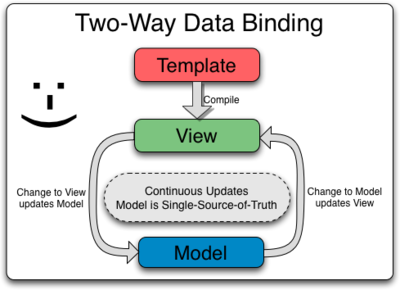
\includegraphics[scale=0.65]{obrazky/twoway_databinding}
\par\end{centering}
\caption{Diagram obousměrného data bindingu knihovny AngularJS \cite{angular} \label{fig:twoway-angular}}
\end{figure}
\FloatBarrier

AngularJS také řeší správu závislostí jednotlivých částí aplikace, a to podle principu \textit{Dependency Injection}, který odebírá třídám zodpovědnost za získání závislostí. Řešení je její převedení na standardizovaný kontajner, který závislosti třídám předává při jejich vytvoření. Framework také poskytuje rozhraní pro sledování změn v modelu (tzv. watchers) a celkově usnadňuje obsluhu událostí. Další z oblíbených vlastností je možnost definice vlastních znovupoužitelných HTML komponent zde nazvaných direktivy. Direktiva v AngularJS je fakticky vlastní HTML element, který zobrazovací logika frameworku převede na běžné HTML dle definice direktivy \cite{angular}.

\subsection{React}
\label{sec:react}
Po nějaké době používání velkých javascriptových MVC frameworků typu AngularJS, které řeší vše uvnitř webového prohlížeče, se začaly projevovat nevýhody toho přístupu. S rozmachem node.js přicházely názory, že je nutné část logiky přesunout zpět na server. Vývojáři moderních webových aplikací, kteří nechtěli používat klasické MVC frameworky, hledali framework vhodný pro jednoduší webové aplikace. Takový, který by řešil jen pohledovou vrstvu, která po přesunutí aplikační logiky na server zůstane webovému prohlížeči. Objevili React. React, což je knihovna pro vytváření uživatelského rozhraní, která řeší pouze pohledovou vrstvu aplikace, tedy jen pomyslné písmeno V z principu MVC. Samotný framework React vznikl jako opensource projekt již v květnu 2013 ve společnosti Facebook. V době vydání byl komunitou přijat převážně negativně, dokonce tak negativně, že společnost Facebook uvažovala o jeho stažení. K tomu ale nakonec nedošlo. React byl jako takový doceněn až v roce 2015, kdy začal být hojně používán pro programování isomorfních webových aplikací. Tedy takových, které používají jazyk Javascript i na serveru. V této době začínali vývojáři postupně opouštět velké monolitické MVC frameworky a přecházet k velmi modularním javascriptovým aplikacím, složených z mnoha knihoven. Dnes má React více než 6000 commitů a kolem 700 přispěvovatelů na serveru Github a je tak jedním z nejoblíběnějších a nejaktivnějších git repozitářů. Úspěch frameworku React také započal opensourcování dalších interních javascriptových projektů společnosti Facebook, jako například immutable.js nebo React Native (pro mobilní telefony). Dnes jsou nástroje společnosti Facebook jedněmi z nejpoužívajších při vývoji moderních webových aplikací v Javascriptu \cite{spa_horyna} \cite{react} \cite{react_book}.

React vývojářům umožňuje kompletní abstrakci od DOM. Strukturu stránek definujeme pomocí sady komponent, kterým dodáme data a framework se již postará o jejich správné vykreslení. Podstatou frameworku je rozbití všech DOM elementů na co nejmenší, nezávislé části (komponenty), které mají vlastní stav a vlastnosti. Tím je zajištěno, že jakákoliv změna jedné části aplikace neovlivní žádnou jinou část. React preferuje HTML v kódu, což je velký rozdíl oprati ostatním frameworkům, kteří naopak vkládájí kód do HTML. Javascript je totiž mnohem expresivnější jazyk než HTML, proto se vyplatí používat pouze jej. React proto zavedl speciální rozšíření Javascriptové syntaxe znamé JSX. S ní lze zapisovat komponenty knihovny React pomocí syntaxe velmi podobné HTML. Na ukázce kódu je vidět definice jednoduché komponenty s jedním div elementem obsahujícím text Hello World v JSX \cite{react} \cite{react_book} \cite{react_intro}.

\begin{lstlisting}[language=Javascript,caption={Ukázka definice Hello World komponenty v JSX}]
 var Greeting = React.createClass({
    render: function() {
      return (
         <div className="title">Hello World</div>
       );
   }
 });
\end{lstlisting}

Framework React je také většinou součástí isomorfních webových aplikací, proto je podrobně popsán v kapitole \hyperref[sec:react]{4.4.5}, která se jim podrobně věnuje.

\section{Možnosti testování}
Díky stále narůstající komplexitě webových aplikací, hraje čím dál tím větší roli jejich testování. 
Nejinak je tomu i v Javascriptu, kde testování probíhá pomocí platformy node.js, pro kterou dnes existuje velké množství různých testovacích nástrojů. Obecně se v Javascriptu používají následující dva základní typy testů \cite{zdrojak_jstesting} \cite{jstesting}.

\begin{itemize}
\item \textbf{Unit testy} se používají pro testování izolované části kódu, nejčastěji metody třídy. Závislosti na ostatní objekty jsou nahrazeny falešnými (mock) objekty, které požadované chování simulují. Jednotkové testy jsou díky tomu rychlé a podporují tvorbu kvalitního kódu \cite{zdrojak_jstesting}.
\item \textbf{Integrační testy} prověřují, zda jednotlivé části systému spolu správně fungují. Na rozdíl od unit testů mohou používat externí zdroje (např. databáze), díky čemuž je však jejich běh pomalejší \cite{zdrojak_jstesting}. 
\end{itemize}

\vspace{3mm}
Oba druhy testů jsou stejně důležité a neměly by v dnešní moderní webové aplikaci chybět. Absence unit testů většinou značí otestování aplikace jen pro základní scénáře. Chybí-li v aplikaci integrační testy, není zajištěno, že jednotlivé části aplikace komunikují správně, například, že databáze vždy vrátí to co v aplikaci očekáváme \cite{zdrojak_jstesting} \cite{jstesting}.
\subsection{Unit testy}
Pro unit testování jsou nejpopulárnější frameworky \textit{Mocha} \cite{mocha}, \textit{Jasmine}, nebo \textit{Vows}. Pro integrační testování aplikací nad serverovým frameworkem Express je výborný modul \textit{supertest} \cite{supertest}. Pro srozumitelné asertace se zase hodí modul \textit{should.js} \cite{should_js}. Pro mockování\footnote{Nahrazení reálného objektu jeho testovací variantou.} objektů se často používá balíček \textit{SinonJS}. Následující ukázka kódu demonstruje jednoduchý unit test převádění mezer na pomlčky pomocí test frameworku Mocha, který je dostupný pomocí NPM \cite{mocha} \cite{zdrojak_jstesting} \cite{jstesting}.

\begin{lstlisting}[language=Javascript,caption={Ukázka jednoduchého unit testu ve frameworku Mocha \cite{zdrojak_jstesting}.}]
var url = require(process.cwd() + '/lib/filters/url');
describe('url filter', function(){
    it('prevede mezery na pomlcky', function(){
        url('nejaky nazev stranky').should.eql('nejaky-nazev-stranky');
            // výsledek volání funkce url('nejaky nazev stranky') musí být 'nejaky-nazev-stranky'
    })
});
\end{lstlisting}
Node.js sice obsahuje přímo modul assert, který lze pro testování používat, populárnější je však dnes jiný způsob psaní testů, který přinesl nástroj Should.js, pomocí kterého lze psát mnohem čitelnější testy. Používájí se dvě základní funkce \textit{describe()} a \textit{it()}. Funkce \textit{describe()} slouží jako kontajner pro samotné testy, které se zapisují dovnitř funkce \textit{it()}. Testovací framework také přidává objekt \textit{should} na všechny použité objekty. Na něm lze volat spoustu asertačních metod. Ukázka 2.13 používá asertační metodu \textit{eq()}, která porovnává dva výsledky. Očekáváme tedy totožné objekty. Celá syntaxe ja navržena tak, aby byly testy co nejlépe čitelné dle metodiky Behaviour Driven Development \cite{jstesting} \cite{should_js}.

\subsection{Integrační testy}
Jak již bylo zmíněno, integrační testy slouží pro ověření komunikace aplikace s externími zdroji, například s databází. Integrační testovaní je v node.js řešeno mimo jiné pomocí knihovny \textit{supertest}, která zajišťuje simulaci zpracování HTTP požadavku. Takový test, ověřující získání všech stránek přes API pages může vypadat například následovně \cite{zdrojak_jstesting} \cite{jstesting}:

\begin{lstlisting}[language=Javascript,caption={Ukázka integračního testů pomocí frameworku supertest \cite{zdrojak_jstesting}.}]
var supertest = require('supertest');
var app = require(process.cwd() + '/app');

describe('API pages', function(){
    describe('GET /api/pages', function(){
        it('vrati seznam vsech polozek v databazi', function(done){
            supertest(app)
                .get('/api/pages')
                .expect(200)
                .end(function(err, res) {
                    res.body.length.should.eql(2); // očekáváme dva záznamy
                    res.body[0].should.include({url:'abc'}); //první z nich musí obsahovat klíč url s hodnotou 'abc'
                    done();
                });
        });
    });
});
\end{lstlisting}

Funkci \textit{supertest} nejprve předáme konfiguraci webové aplikace z frameworku Express a pomocí metody \textit{get()} simulujeme GET požadavek na předané URL. Funkce \textit{except()} ověřuje stavový kód HTTP požadavku a v metodě \textit{end()} poté provádíme testování samotné odpovědi serveru \cite{zdrojak_jstesting} \cite{jstesting}. Zde je opět použit testovací framework should.js, ověřujeme zda odpověď obsahuje právě dva záznamy a první prvek obsahuje klíč \textit{url} s hodnotou \textit{abc} \cite{should_js}.  Často je také potřeba před samotným testováním nejprve uložit do databáze nějaká testovací data, k tomu slouží metoda \textit{beforeEach()}, která proběhne vždy před každým testem. Existuje také podobná metoda \textit{afterEach()}, která naopak proběhne po každém testu \cite{zdrojak_jstesting} \cite{jstesting}. Oblíbené je také provádění integračních testů pomocí automatizace webového prohlížeče, například pomocí rodiny nástrojů Selenium \cite{selenium}.

Spouštění a zobrazování výsledků všech testů pro jazyk Javascript většinou zajišťuje nějaký task runner, například Grunt, Gulp nebo NPM (viz \hyperref[sec:task_runners]{4.4.7}) \cite{jstesting}.

\subsection{Testování React komponent}
V dnešní době složitých webových aplikací je vhodné testovat také frontendové frameworky, například již zmiňovaný React. Stejně jako integrační testy je vhodně test frontendového kódu spouštět přímo v prohlížeči, a to nejlépe rovnou v několika nejpoužívanějších z nich. To je práce, kterou zajišťuje testovací nástroj \textit{Karma}. Karma je frontendový test-runner, který umí importovat testy z běžně používaného testovacího frameworku (například Jasmine a další), které potom v definovaných prohlížečích automaticky spouští \cite{karma}. Dalším vhodným nástrojem pro testování React aplikací je \textit{Enzyme} vyvinutý ve společnosti AirBnB. Jeho výhody spočívájí v jednoduché syntaxi testů a schopnosti simulace uživatelských událostí \cite{enzyme} \cite{testing_react}. Chceme-li otestovat, zda se React komponenta správně zobrazuje, je třeba jí nejprve vykreslit. Nástroj Enzyme k tomu poskytuje dvě metody. První, \textit{shallow()} vykresluje pouze do virtuálního DOM a je vhodnější spíš pro jednoduché unit testy. Metoda \textit{mount()} již do testování zapojuje i DOM webového prohlížeče. Jednoduchý test, který u aplikace ověřuje správnost hlavního nadpisu (h1), může vypadat například takto \cite{enzyme} \cite{testing_react}:

\begin{lstlisting}[language=Javascript,caption={Ukázka testu React komponenty App \cite{testing_react}}]
const assert = require('assert');  
const App = require('../../../public/components/app.jsx');  
const React = require('react');  
const enzyme = require('enzyme');

describe('#app component', () => {  
    it('should render header', () => {
        const app = enzyme.mount(
            <App />
        );
        assert.equal(app.find('h1').text(), 'Hello world');
    });
});
\end{lstlisting}